\documentclass[letterpaper, 12pt]{article}
\usepackage{graphics} 
\usepackage{amsmath} 
\usepackage{amsthm}
\usepackage{amssymb}
\usepackage{optidef}
\usepackage{xcolor}
\usepackage{derivative}
\usepackage[backend=biber]{biblatex}
\usepackage{cleveref}
\addbibresource{surface_planner.bib}

\usepackage{color}
\def\startmodif{\color{blue}}
\def\stopmodif{\color{black}\normalcolor}
\def\citationneeded{\color{magenta}{\small{[citation needed]}}\normalcolor}
\def\uterrain{_{\text{terrain}}}
\def\usurface{_{\text{surface}}}
\def\xij{\mathbf{x}_{ij}}
\def\zsij{z_{(s) i,j}}
\def\ztij{z_{(t) i,j}}
\def\zij{z_{i,j}}
\def\Zij{Z_{i,j}}
\newcommand{\dac}[1]{\color{red}#1}
\newcommand{\mls}[1]{\color{teal}#1}
\newcommand{\diff}[1]{\text{diff( }#1\text{ ) }}

\newtheorem{theorem}{Theorem}[subsection]


\title{Improving RRT* for a UAV with Dynamic Constraints in 3 Dimensions Using an Optimal Embedded Surface}
\author{Mike L. Sutherland, David A. Copp}

\begin{document}

\maketitle

\section{Introduction}
Unmanned Aerial Vehcles (UAVs) are increasingly used in many applications. Much attention has been devoted to Path Planning for UAVs, especially those with difficult dynamic constraints, such as fixed-wing aircraft. Computing safe and optimal paths for UAVs with dynamic constraints can be computationally complex and can require long planning times, especially if the configuration space has more then two dimensions. These computational challenges hinder the ability of fast-moving vehicles to find collision-free paths in real time. \citationneeded Therefore, some of the most significant considerations when formulating and solving these path planning problems are computational complexity, planning time available, and desired degree of constraint satisfaction and optimality. 

We can clearly see this tradeoff at play in the family of algorithms based on the Rapidly-Exploring Random Tree (RRT) \cite{lavalle2006}. RRT algorithms are frequently used for motion planning in high-dimensional spaces because of their ability to compute paths that are approximately optimal. In fact, as more samples are drawn from the configuration space, the RRT path approaches an optimal path. Because drawing each sample takes some finite time, plans generated by RRT algorithms are improved if the samples are drawn quicker. These qualities make RRT and its derivatives like a Monte Carlo method for a specific class of non-convex problem: the planning-with-constraints problem.

In thinking about the RRT planner as a non-convex optimization, we ask: can we reduce the size of the configuration space in an optimal way to reduce computational complexity and resulting planning times? In this work, we propose a strategy to reduce the 3-dimensional configuration space of a fixed-wing UAV to a 2-dimensional configuration space by solving a convex problem. 


{\dac This is sounding really good. We should include several references related to RRT*, its computational complexity, and what clever solutions people already use to compute solutions efficiently. Then say that we propose a method to reduce complexity by collapsing a 3-dimensional search space into a 2-dimensional search space that is parameterized by the dynamics constraints at each node, which is a new way to formulate the problem and efficiently find solutions, particularly for dynamics-constrained path planning problems in 3-dimensions. etc. etc. Something like this with the specific details and contributions of this work.}


\section{\startmodif Problem Formulation \stopmodif}

We consider the problem of computing safe and optimal paths for a dynamics-constrained vehicle in a 3-dimensional configuration space (C-space), parameterized by the triplet $(x,y,z) \in \mathbb{R}\times \mathbb{R} \times Z$, where $Z \subset \mathbb{R}$ is simply connected and lower-bounded with its lower bound given by some function $f_{\text{terrain}}(x,y)$. The physical interpretation of such a space is a 3-D volume, open on top and closed on the bottom by some continuous terrain, whose height is given by $f_{\text{terrain}}$. 

The first two dimensions of the configuration space are represented by a square grid with each cell having length and width $d$. Therefore, the first two dimensions of the configuration space are fixed in place as grid lattice points. The last dimension in the $z$ direction is some real valued altitude, belonging to $Z$. We call such a point $z$.

It is important to distinguish between the 2D planning space and the 3D robot space. We denote a 2-dimensional point $\xij$ using some $(i,j) \in (M \times N)$ where $M, N$ are simply connected subsets of $\mathbb{Z}$. Attached to each grid point are heights. We call the height of the terrain at some grid point at $\xij$ by $\ztij$. The height of the vehicle is simply $z_{i,j}$. We pre-compute the altitude of a "surface" on which to plan; this surface altitude is called $\zsij$. Thus, for any $\xij$ in the grid, we have some altitudes and distances, each of which shares the same $\xij$, but with differing altitudes in $Z$.
\section{Main Results}

Our task is to find a set of altitudes for each grid point $\xij$, with the following properties. 
\begin{itemize}
\item{All are higher than the terrain by more than some constant buffer, $h_{\text{buffer}}$:
\begin{equation}
\zsij - \ztij \geq h_{\text{buffer}}
\label{eq:buffer}
\end{equation}
}
\item{All are higher than some minimum altitude $h_{\text{min}}$:
\begin{equation}
\zsij \geq h_{\text{min}}
\label{eq:altmin}
\end{equation}
}
\item{The difference in altitude between a grid point and each of its neighbors is less than some constant slope $v_{\text{max}}$:
\begin{equation}
\begin{aligned}
    | \zsij - z_{(s) i-1, j} | &\leq v_{\text{max}} \forall (i, j) \in (M_{\backslash  \{0\}}, N) \\
    | \zsij - z_{(s) i, j-1} | &\leq v_{\text{max}} \forall (i, j) \in (M, N_{\backslash  \{0\}})
\end{aligned}
\label{eq:slope}
\end{equation}
The physical interpretation of this relation is a maximum 1st spatial derivative, $\left|\pdv{z}{ \mathbf{x} } \right| \leq v_{\text{max}}$, and label it with an operator:
\begin{equation}
    \diff{z_s, i} = | \zsij - z_{(s) i-1, j} |
    \label{op:diff}
\end{equation}
\mls{So, I wonder what the least-clunky way is to define this set $(M_{\backslash  \{0\}}$. What I really mean is $M$ minus its first element. And, how can I better state this diff operator? It's basically straight out of numpy, but I don't know if there is a widely accepted mathy definition for it.}
}
\item {The difference in altitude difference between a grid point altitude difference and each of its neighbors is less than some constant, $a_{\text{max}}$. Using \cref{op:diff}:
\begin{equation}
    \begin{aligned}
        \diff{\diff{ z_s, i}} &\leq a_{\text{max}} \forall (i, j) \in (M_{\backslash  \{0, 1\}}, N) \\
        \diff{\diff{ z_s, j}} &\leq a_{\text{max}} \forall (i, j) \in (M, N_{\backslash  \{0, 1\}})
    \end{aligned}
    \label{eq:acceleration}
\end{equation}
The physical interpretation of this relation is a maximum 2nd spatial derivative, $\left| \frac{\partial^2 z_{(s)}}{\partial \mathbf{x}^2} \right| \leq a_{\text{max}}$.
}
\end{itemize}
These constraints amount to a set of "surfaces" of safe altitudes, onto which quickly computed plans in $X,Y$ can be projected. We choosing the best surface from this set by solving the convex optimization problem.

\subsection{Optimal Embedded Surface}

\begin{theorem}
    For a configuration space in $\mathbb{R} \times \mathbb{R} \times Z$, where $Z \subset \mathbb{R}$ is simply connected and lower bounded, there exists an infinte number of sets of points $(x_ij, y_ij, z_ij)$, with each set having properties \cref{eq:buffer,eq:altmin,eq:slope,eq:acceleration}.
\end{theorem}

\begin{proof}
    Let $\mathcal{X}$ be a finite collection of grid points $\mathcal{X} = \{\xij | i \in M, j \in N\}$. Each grid point $\xij$ has a corresponding set of altitudes, $\Zij$, which is lower bounded and simply connected, with a lower bound given by $\ztij = f_{\text{terrain}}(\xij)$. We call the set of altitude sets $\mathcal{Z}$.
    
    Let us define a space defined by the constraints given by \cref{eq:buffer,eq:altmin}:
    \begin{align}
        B_{i,j} &= \{ {\zij | \zij - \ztij \geq h_{\text{buffer}}, \zij \in \Zij} \} \\ \nonumber
        L_{i,j} &= \{ {\zij | \zij \geq h_{\text{min}}, \zij \in \Zij} \} \\ \nonumber
        C_{i,j} &= \Zij \backslash (B_{i,j} \bigcup L_{i,j}) \in \mathcal{C}
    \end{align}
    {\mls can I distribute the complement operation like this?}

    The set $\mathcal{C}$ is also lower bounded and simply connected, and it contains all possible surfaces (even those that violate derivative constraints).

    {\mls for existence, I just have to prove that the set of surfaces matching derivative constraints is a non-null subset of $\mathcal{C}$. Then I can say that there is some minimum altitude surface in that collection that can be found by solving the optimization problem. Not sure how I would prove that, other than to say that the combination of constriants/costs is DCP}
\end{proof}
We can formulate the problem of finding an optimal embedded surface as a convex optimization problem that can be solved before, and used in, the path-planning algorithm.

This convex optimization problem can be written as 

\begin{mini!}
    {\startmodif z \stopmodif}{J = z}
    {\label{eq:Example1}}
    {}
    \addConstraint{ z }{ \geq z_\text{min} }
    \addConstraint{ z - z_\text{gap} }{ \geq z_\text{obs} }
    \addConstraint{ \pdv{z}{x} }{ \leq v_\text{max} }
    \addConstraint{ \frac{\partial ^2 z}{x^2} }{ \leq a_\text{max} } % 2nd partial derivative package does not work in mini! environment
\end{mini!}
where $z$ is the vehicle height and $z_\text{obs}$ is the obstacle height. $v_\text{max}$ is the maximum climb rate of the vehicle, $a_\text{max}$ is the maximum vertical acceleration of the vehicle, and $z_\text{gap}$ is the minimum gap between the vehicle height and the height of an obstacle.

{\dac Describe the optimization variables and constraints. Should be as general as possible but could then specialize for a UAV, describing the dimensionality of the variables and their physical meaning.}

\startmodif Solving the convex optimization problem \eqref{eq:Example1} \stopmodif gives us an optimal cost for each point in the configuration space. We can think of this cost as an ``elevation.'' Indeed, in the UAV inspection task, we are trying to fly as low as possible. Then, computing a plan between $x_1$ and $x_2 \in X$ and projecting onto $\mathcal{X}$ will produce a valid plan which will direct the UAV to a safe and optimal height, even under the vehicle's vertical climb and acceleration constraints.

\subsection{\startmodif Reduced Complexity Path Planning Algorithm \stopmodif}

At a high level, the steps of the algorithm are as follows:

\begin{itemize}
    \item Solve the convex problem \eqref{eq:Example1}
    \item Use the solution to the convex problem to inform the cost function of the RRT*
    \item Solve a 2-D RRT* problem with an altered cost function, $c(\bar{x})$, to obtain an optimal course over the sheet.
    

\end{itemize}


{\dac Discuss how to choose cost function of RRT*}

However, we can also improve our RRT by altering its cost function with an additional heuristic informed by this new elevation data. We use the RRT* algorithm, but replacing the standard euclidean cost function

\begin{equation}
c_\text{eu}(\bar{x}_1, \bar{x}_2) = |(x_2 - x_1)|
\end{equation}


With a new cost function. Let $l_{12}$ be a collection of points in $X$, each of which is some distance from a straight line from $x_1$ to $x_2$,

\begin{equation}
l_{12} = \{x \in X | \min(|x - l_{12}|) \leq u \},
\end{equation}

where $u \geq d$. Algorithms such as Bresenham's Straight Line algorithm can be used to compute such collections quickly. The z-values of these points (in $\mathcal{X}$-space) are their ``elevations'' on the sheet. Call this collection of z-values $\mathcal{Z^\text{line}}$. We then plan in $X$ using the cost function
\begin{equation}
c_\text{sheet}(x_1, x_2) = |x_2 - x_1| + \gamma_z \cdot |x_2 - x_1| \cdot \sum^k_i({\frac{z_i}{k}})
\end{equation}

\footnote{
Probably, we need to prove that this cost function forms a metric space $(\mathcal{X}, c)$: positivity, symmetry,  triangle inequality. I think I can use some clever properties of each term and the composition thereof to do this succinctly.}

Where $\gamma_z$ is a scaling factor, $|x_2-x_1|$ is the $\mathbb{R}^2$ distance between the points, and $z_i$ is the elevation of the $i$ th point in a collection of $k$ points formed by the line $l_{12}$. Note that when the scaling factor $\gamma_z=0$, $c_\text{sheet}$ reduces to $c_\text{eu}$. This factor represents a cost penalty on the elevation of each point between the points $x_1$ and $x_2$. 

\section{Numerical Example}
\begin{figure}
    \centering
    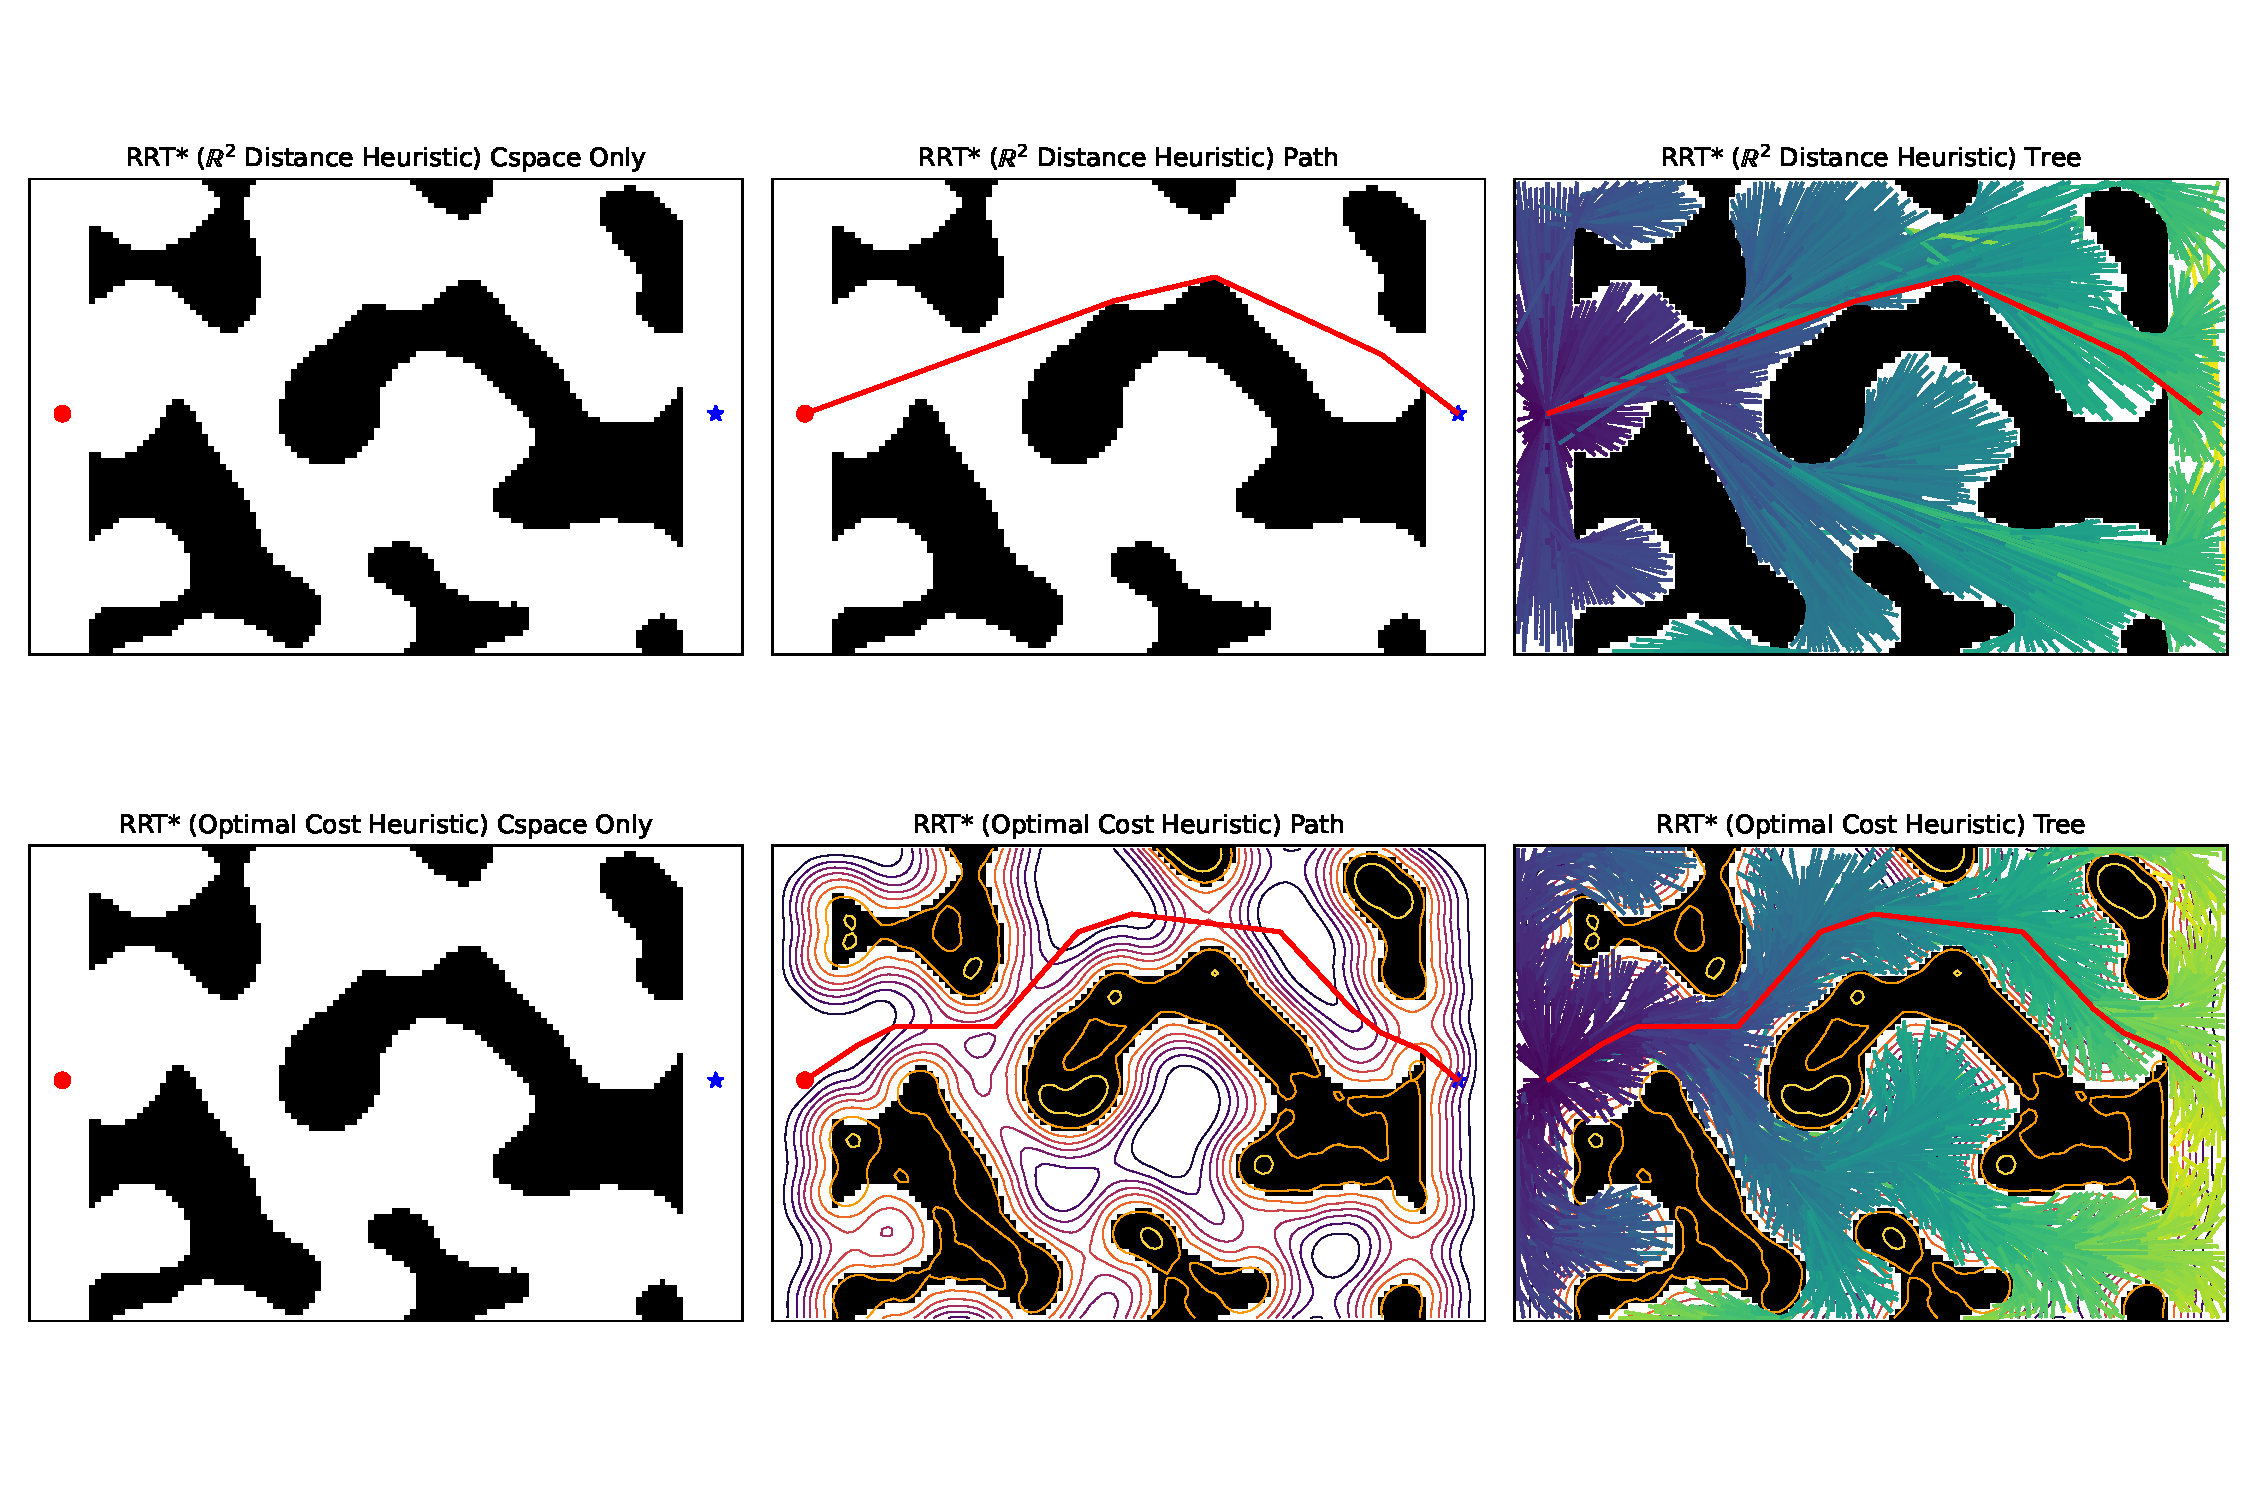
\includegraphics[width=0.9\linewidth]{./figures/rrt_surface_fig.pdf}
    \caption{A comparison between the RRT* algorithm (n=4000) run with the standard Euclidean cost function (top row) and a cost function with a penalty on the elevation of the point in the $z$-dimension (bottom row). The first column shows the configuration space, which is the same between both planners. The second column (in the second row) shows the contour lines of $z$-elevation of the computed surface, with the obstacles treated as elevated terrain. Finally, the tree and computed paths are shown. We see a more cautious path, in the bottom row, since $z$-elevation is punished in the RRT* cost function and the elevation is higher near obstacles.}
\end{figure}

\section{Comments}
{\mls
My intuition says that the RRT cost function is isometric with the distance metric of the configuration space. This *seems* like a prerequisite for the RRT to approach optimality. And, that changes to the RRT cost function that preserve isometry between the two metrics are changes which preserve the property of the RRT which results in the RRT approaching optimality.

Like, that isometry between a cost functions $c$ and $c_\text{eu}$, is a *necessary* and *sufficient* condition for the RRT to find an optimal path through some type of euclidean C-space...

I've tried looking at papers that would explain this or proofs, but everything is so applied -- most use variants of the euclidean cost (if they change it at all), and they do not discuss the properties of the cost function that they use.

I think there is something very interesting and important about the cost function of the RRT that relates to its ability to solve this non-convex problem almost - optimally. Most papers are focused on getting the solution to converge faster on the euclidean metric, but hardly any are looking at the properties of the cost function! EDIT: there is one that uses artificial potential fields; I think it could be very exciting to explore that more formally. I think it's crucial for actually explaining how solving the first convex problem, then using that solution inside of the RRT cost, makes the RRT converge to a better solution -- one which is informed by the information obtained from the convex problem.}

\printbibliography

\end{document}
